\documentclass[
    english,
    accentcolor=9c,
    design=2023,
    logofile=images/hulogo.pdf,
]{tudabeamer}

\usepackage[english]{babel}
\usepackage[autostyle]{csquotes}
\usepackage{bookmark}
\usepackage{enumitem}
\usepackage{eurosym}
\usepackage{multirow}
\usepackage{siunitx}

\newcommand*{\code}[1]{\texttt{#1}}

\title[LikertShift]{LikertShift - An Input Device for Recording Cycling Subjective Experiences}
\subtitle{Bachelor's Thesis Defense}
\author{Max Schlecht}
\department{Human Computer Interaction}
\institute{Humboldt-Universität zu Berlin}

\date{2025-08-13}

\AtBeginSection{\sectionpage} % Enable section pages

\makeatletter
\patchcmd{\beamer@sectionintoc}
{\vfill}
{\vskip\itemsep}
{}
{}
\makeatother

\let\footnoterule\relax
\renewcommand\thefootnote{}
\setbeamerfont{footnote}{size=\tiny}

\begin{document}

\maketitle

\tableofcontents

\section{Motivation}

\begin{frame}{Motivation}
    \centering
    \includegraphics[height=0.35\linewidth]{images/vemotion.png}
    \footnotetext{VEmotion (Bethge et al.) \quad \url{https://doi.org/10.1145/3472749.3474775}}
\end{frame}

\begin{frame}{Motivation}
    \begin{columns}[onlytextwidth,c]
        \column{.5\linewidth}
        \centering
        \includegraphics[height=0.55\linewidth]{images/button_device.png}
        \footnotetext{Analysis of Overtaking Maneuvers \ldots (L\'{o}pez et al.)}
        \footnotetext{\url{https://doi.org/10.1145/3472749.3474775}}
        \column{.5\linewidth}
        \centering
        \includegraphics<2>[height=0.55\linewidth]{images/brotate.png}
        \footnotetext<2>{Brotate and Tribike \ldots (Wo\'{z}niak et al.)}
        \footnotetext<2>{\url{https://doi.org/10.1145/3472749.3474775}}
    \end{columns}
\end{frame}

\section{Prototype Design}

\begin{frame}{Design Requirements}
    \begin{enumerate}[label=\textsf{DRQ\arabic*}, left=1em .. 4.5em]
        \item<1-> \textbf{Intuitive}

            Using the prototype should be intuitive.

            \note<1>{- Prototyp moeglichst einfach zu benutzen + offensichtlich}

        \item<2-> \textbf{Robust}

            Minimal user intervention and maintenance.

            \note<2>{
                - wartungsarm (Batteriewechsel, langsame Abnutzung)\\
                - Prototyp sollte bei normaler Nutzung nicht kaputt gehen\\
                - in der Lage Umgebungsbedinungen (Regen, Feuchtigkeit, Temperaturschwankungen) auszuhalten
            }

        \item<3-> \textbf{Safe}

            Uncompromising to the user's safety.

            \note<3>{
                - Sicherheit beim Fahrradfahren nicht eingeschraenkt\\
                - gewisse Ablenkung durch Bewerten ist immer gegeben
            }

        \item<4-> \textbf{Affordable}

            Total cost < \euro25.00.

            \note<4>{
                - guenstig, festgelegter maximalpreis von 25 euro\\
                - erschien mit herstellungsmeth., art von hardware erreichbar
            }

        \item<5-> \textbf{Easy to Reproduce}

            Manufactured and assembled with standard components and tools.

            \note<5>{
                - einfach nachzubauen\\
                - benoetigte bauteile + werkzeuge sollten standardmaessig verfuegbar sein
            }
    \end{enumerate}
\end{frame}

\begin{frame}{LikertShift Prototype}
    \begin{columns}[onlytextwidth,c]
        \column{.5\linewidth}
        \centering
        \includegraphics[height=0.7\linewidth]{../images/likertshift_assembled.jpg}
        \column{.5\linewidth}
        \centering
        \includegraphics[height=0.7\linewidth]{../images/likertshift_mounted.jpg}
    \end{columns}
\end{frame}

\begin{frame}{How does it work?}
    \framesubtitle{Mechanics}
    \begin{columns}[onlytextwidth,c]
        \column{.5\linewidth}
        \centering
        \includegraphics[height=0.7\linewidth]{../images/cad_rotator_head.jpg}
        \column{.5\linewidth}
        \centering
        \includegraphics[height=0.7\linewidth]{../images/cad_ramped_track.jpg}
    \end{columns}
\end{frame}

\begin{frame}{How does it work?}
    \framesubtitle{Electronics}
    \begin{columns}[onlytextwidth,c]
        \column{.5\linewidth}
        \centering
        \includegraphics[height=0.7\linewidth]{../images/likertshift_pcb.jpg}
        \column{.5\linewidth}
        \centering
        \includegraphics[height=0.7\linewidth]{../images/cad_pcb_compartment.jpg}
    \end{columns}
\end{frame}

\begin{frame}{How does it work?}
    \framesubtitle{Software}
    \begin{columns}[onlytextwidth,c]
        \column{.25\linewidth}
        \centering
        \includegraphics[height=1.35\linewidth]{../images/app_map_screen.jpg}
        \column{.25\linewidth}
        \centering
        \includegraphics<2->[height=1.35\linewidth]{../images/app_routes_screen.jpg}
        \column{.25\linewidth}
        \centering
        \includegraphics<3->[height=1.35\linewidth]{../images/app_devices_screen.jpg}
        \column{.25\linewidth}
        \centering
        \includegraphics<4->[height=1.35\linewidth]{../images/app_tlx_survey.jpg}
    \end{columns}
\end{frame}

\section{Study Design}

\begin{frame}{Study Design}
    \textbf{What methods are we comparing?}
    \pause

    \quad $\Rightarrow$ \;Audio Recording, Manual Mapping, LikertShift
    \pause

    \vspace*{1em}
    \textbf{What are we measuring?}
    \pause

    \quad $\Rightarrow$ \;Travel Satisfaction, based on the road
    \pause

    \vspace*{1em}
    \textbf{Route Selection}

    \vspace*{1em}
    \footnotesize
    \centering
    \begin{tabular}{c|c|ccccc|c}
        \multirow{2}{*}{Name} & \multirow{2}{2.4em}{Total\newline} & \multicolumn{5}{c|}{Road Type} & \multirow{2}{4.7em}{Number of\newline}\\
        \cline{3-7}
        &&&&&&&\\[-1em]
        & Length & Road & Bike Path & Mixed Path & Pedestrian Way & Other & Crossings\\[0.15em]
        \hline
        &&&&&&&\\[-0.8em]
        North & \SI{2589}{m} &  \SI{191}{m} & \SI{480}{m} & \SI{1135}{m} & \SI{359}{m} & \SI{424}{m} & 13\\[0.3em]
        East  & \SI{2007}{m} &  \SI{853}{m} & \SI{465}{m} &  \SI{173}{m} & \SI{181}{m} & \SI{335}{m} & 9\\[0.3em]
        South & \SI{2289}{m} & \SI{1152}{m} & \SI{677}{m} &  \SI{116}{m} &  \SI{47}{m} & \SI{297}{m} & 9\\
    \end{tabular}
\end{frame}

\begin{frame}{Study Design}
    \framesubtitle{Routes}
    \begin{columns}[onlytextwidth,c]
        \column{.5\linewidth}
        \centering
        \includegraphics[height=0.7\linewidth]{../images/wood_planks_path.jpg}
        \column{.5\linewidth}
        \centering
        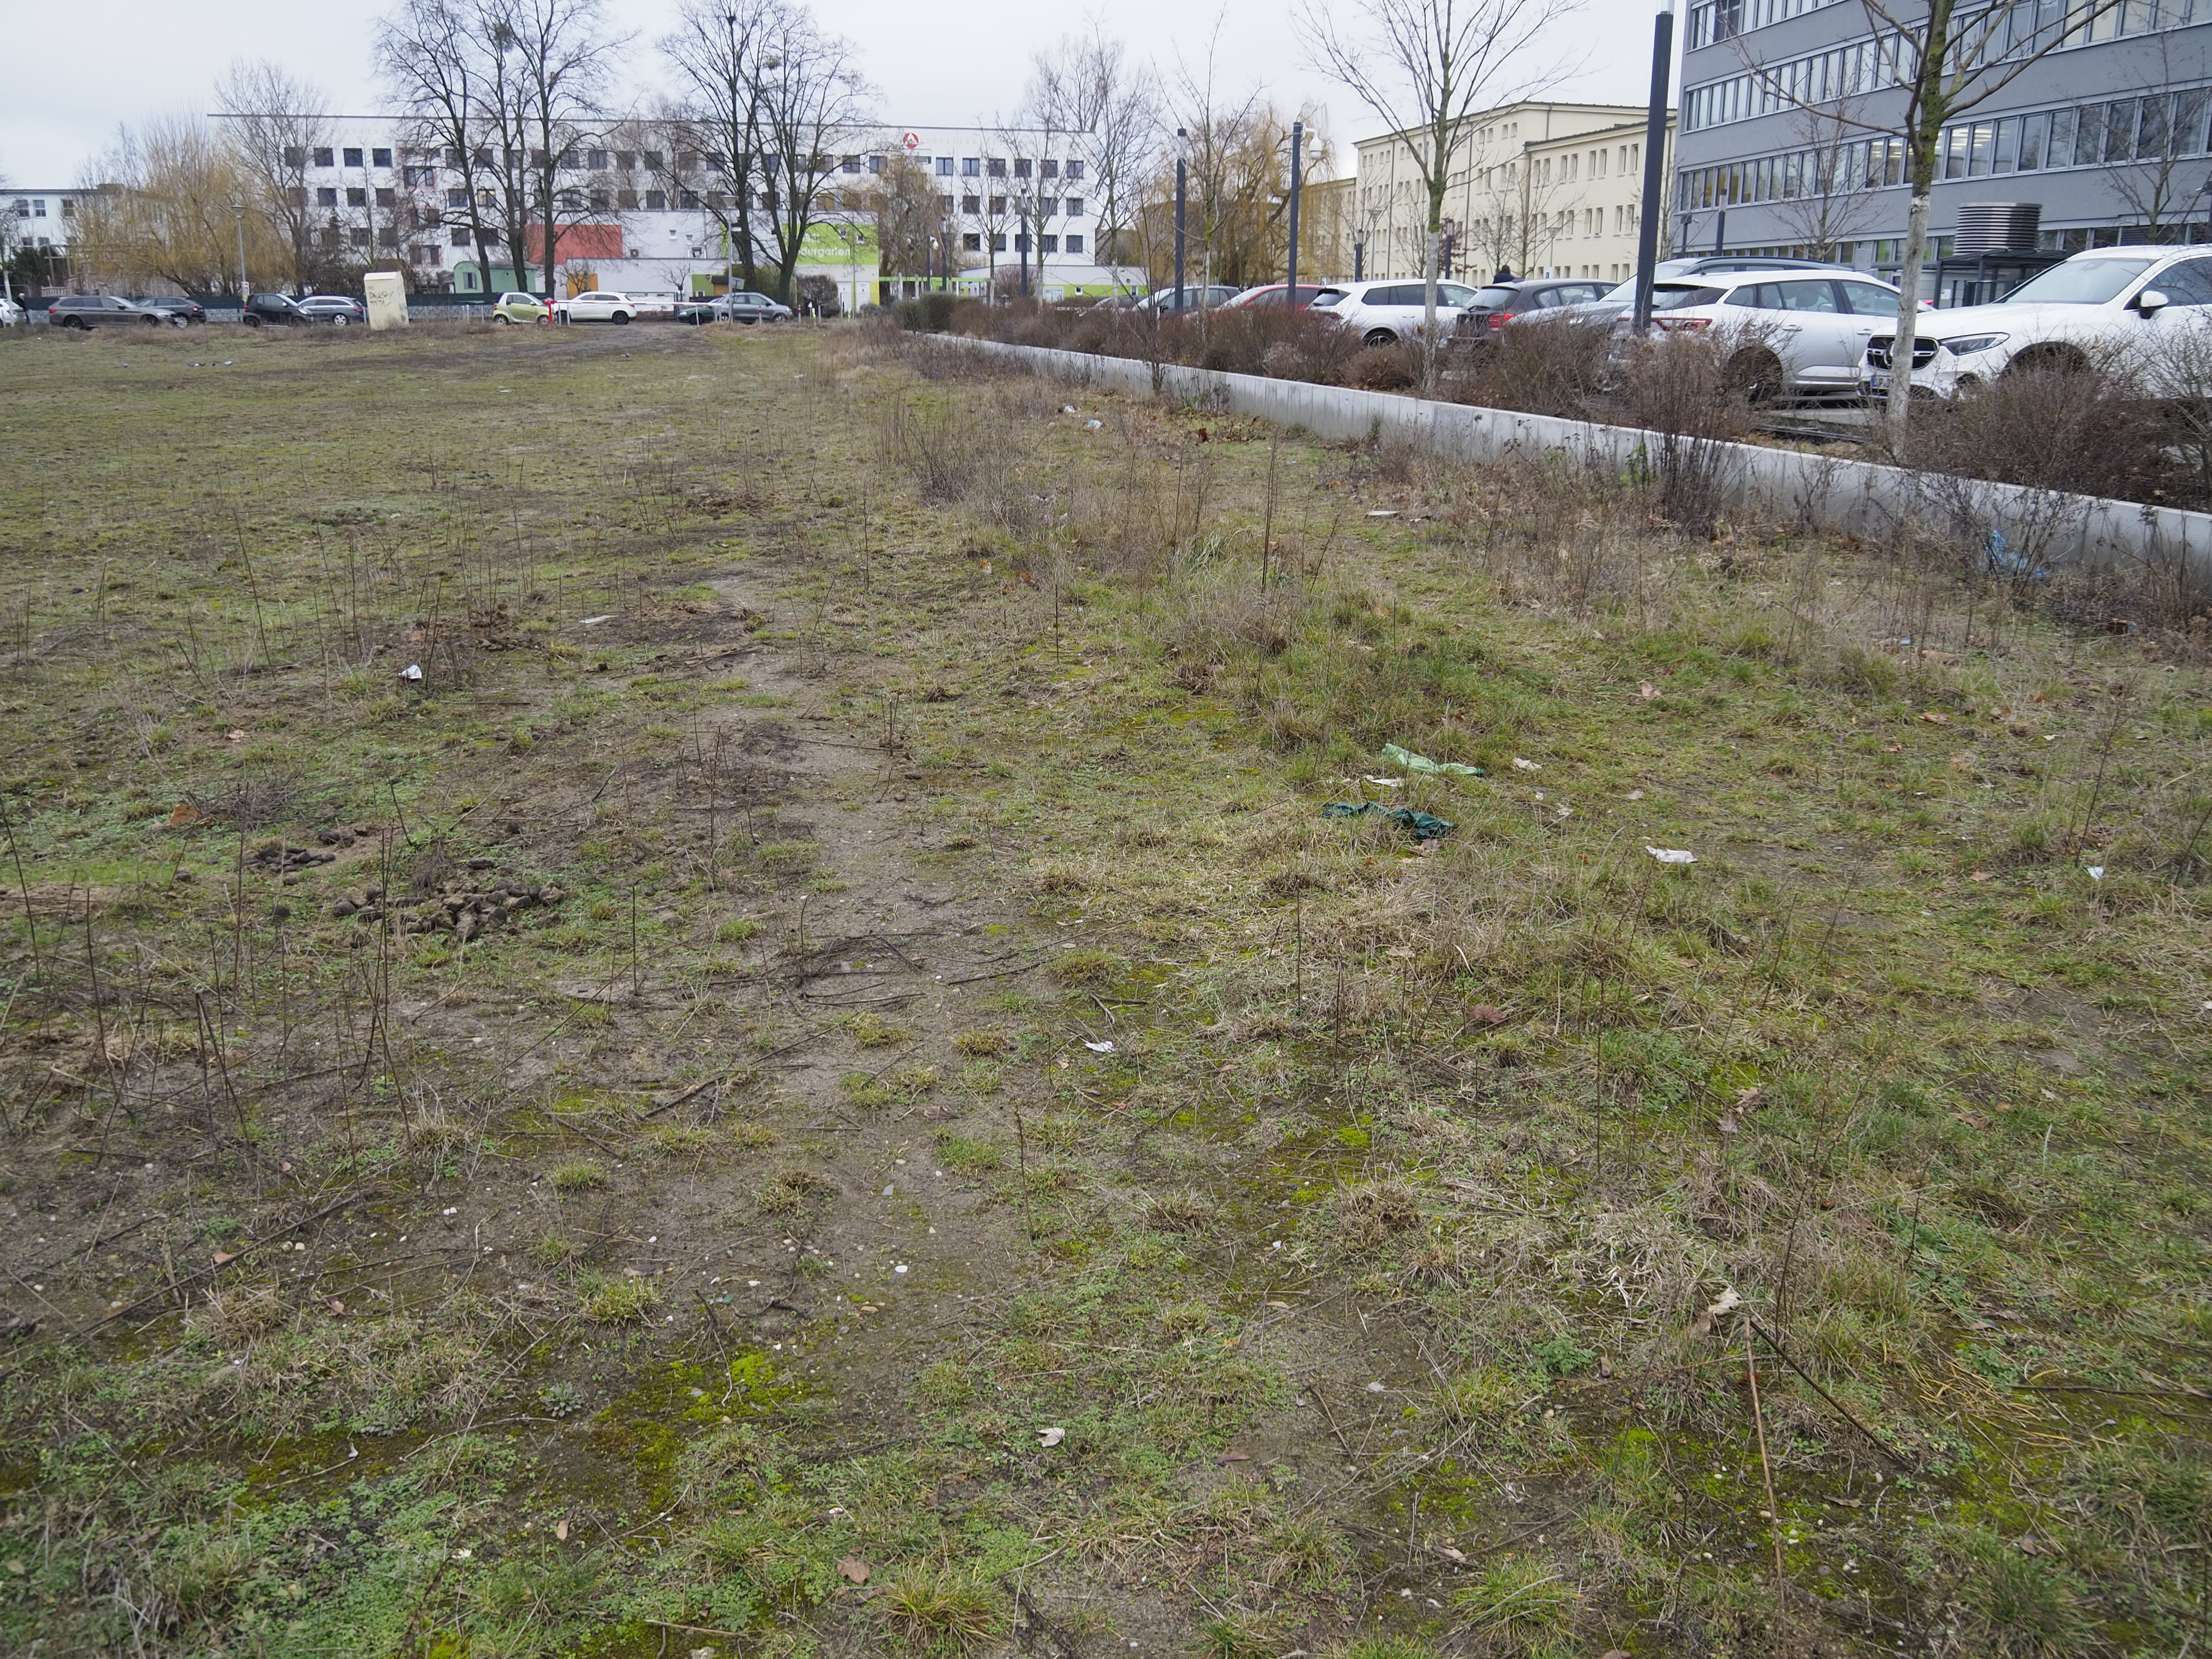
\includegraphics[height=0.7\linewidth]{../images/field_east_route.jpg}
    \end{columns}
\end{frame}
\end{document}
